\section{ХОД РАБОТЫ}

\subsection{Постановка задачи}

Выполнить моделирование случайных чисел с выбранными в соответствии с вариантом
распределениями. Для каждого распределения при m = 2 вывести диаграмму рассеивания, 
на которую нанести $ 100 \dots 500 $ случайных чисел, используя
собственную программу, реализующую предложенный алгоритм, и стандартную программу Matlab.
Собственные программы оформить в виде m-файлов-функций. 

На диаграмму рассеивания двухмерного нормального закона вывести функцию регрессии.

Исследовать изменение диаграмм рассеивания в зависимости от пара-
метров распределений.

\subsection{Теоретические сведения}
\label{sub:theory}

Приведем алгоритм получения двумерной случайной величины $ \bar x = (x_1, x_2) $,
распределённой по \textit{нормальному закону} $ N (\bar a, R) $:

\begin{enumerate}
  \item формируется треугольная матрица следующего вида:
    \begin{align*}
      C = 
      \begin{pmatrix}
        c_{1,1}&0\\
        c_{2,1}&c_{2,2}
      \end{pmatrix}, \\ \\
      \text{где } c_{1,1} = \sqrt[4]{R_{1,1}},
      c_{2,1} = \dfrac{R_{1,2} R_{2,2}}{c_{1,1} \sqrt{R_{1,1}}},
      c_{2,2} &= \sqrt{\sqrt{R_{2,2}} - c_{2,1}^2};
    \end{align*}
    
  \item генерируется двумерная случайная величина $ \bar t = (t_1, t_2) $,
    в ней $ t_1, t_2 $ определяются как одномерные независимые случайные величины, распределенные 
    по нормальному закону $ N(0, 1) $;

  \item результирующая двумерная случайная величина, распределенная по нормальному закону,
    определяется как $ \bar x = (x_1, x_2) = C \bar t + \bar a $. 
\end{enumerate}

\newpage

Для получения случайной величины с многомерным распределением, 
равным \textit{произведению одномерных распределений хи-квадрат}, достаточно
определить искомую случайную величину как $ \bar x = (x_1, x_2, \dots x_n) $,
имеющую n независимых компонент:
\begin{equation*}
  x_i = \sum_{j = 1}^{k}{u^{2}_{j}},
\end{equation*}
\noindent где $ u_{j} $ --- случайные величины с распределением $ N(0,1) $,
$ k $ --- число степеней свободы.

Диаграмма рассеивания --- это рисунок, на который нанесены смоделированные значения
двухмерного случайного вектора.

Функция регрессии для двумерного норамльного распределения определяется 
следующим образом:
\begin{equation*}
y = a_y + r_{x,y} \dfrac{\sigma_y}{\sigma_x}(x - a_x).
\end{equation*}

Здесь $ a_x $, $ \sigma_x $ --- математическое ожидание и среднее квадратичное отклонение аргумента;
$ a_y $, $ \sigma_y $ --- математическое ожидание и среднее квадратичное отклонение функции;
$ r_{x,y} $ --- коэффициент корреляции между аргументом и функцией.

\newpage 

\subsection{Моделирование двумерных случайных величин, \\ распределенных по нормальному закону}

Диаграммы рассеяния случайных величин с двухмерным нормальным законом распределения представлены
на рисунках~\ref{pic:normal_start}--\ref{pic:normal_end}.

\begin{figure}[h!]
  \begin{minipage}[h!]{0.47\linewidth}
    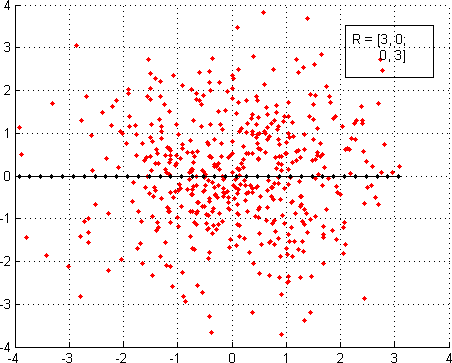
\includegraphics[width=1\linewidth]{pic/normal_our_1}
    \caption{Случайные величины, полученные по реализованному алгоритму,
      при $ R = \big[3, 0, 0, 3 \big] $
  }
    \label{pic:normal_start}
  \end{minipage}
  \hfill
  \begin{minipage}[h!]{0.47\linewidth}
    \vspace{4mm}
    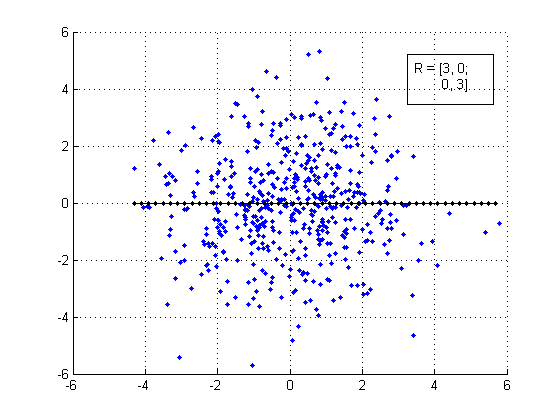
\includegraphics[width=1\linewidth]{pic/normal_matlab_1}
    \caption{Случайные величины, полученные средствами Matlab,
      при $ R = \big[3, 0, 0, 3 \big] $
    }
  \end{minipage}
\end{figure}

\begin{figure}[h!]
  \begin{minipage}[h!]{0.47\linewidth}
    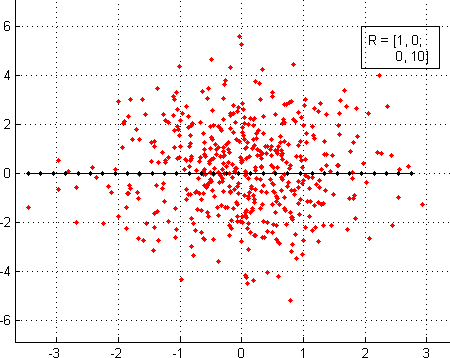
\includegraphics[width=1\linewidth]{pic/normal_our_2}
    \caption{Диаграмма рассеяния случайных величин, распределенных по нормальному закону,
      при $ R = \big[1, 0, 0, 10 \big] $
  }
  \end{minipage}
  \hfill
  \begin{minipage}[h!]{0.47\linewidth}
    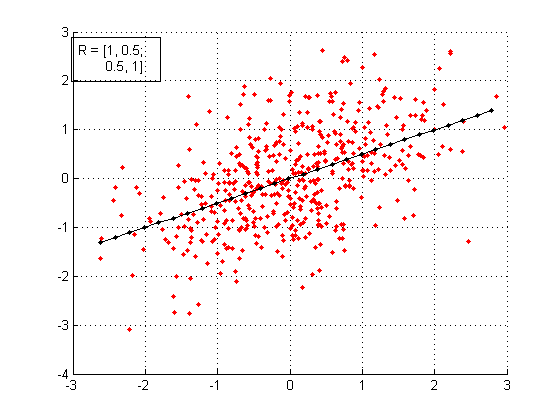
\includegraphics[width=1\linewidth]{pic/normal_our_3}
    \caption{Диаграмма рассеяния случайных величин, распределенных по нормальному закону,
      при $ R = \big[1, 0.5, 0.5, 1 \big] $
  }
  \end{minipage}
\end{figure}

\begin{figure}[h!]
  \begin{minipage}[h!]{0.47\linewidth}
    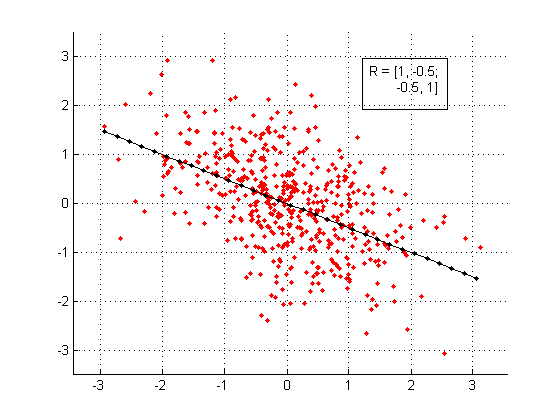
\includegraphics[width=1\linewidth]{pic/normal_our_4}
    \caption{Диаграмма рассеяния случайных величин, распределенных по нормальному закону,
      при $ R = \big[1, -0.5, -0.5, 1 \big] $
  }
  \end{minipage}
  \hfill
  \begin{minipage}[h!]{0.47\linewidth}
    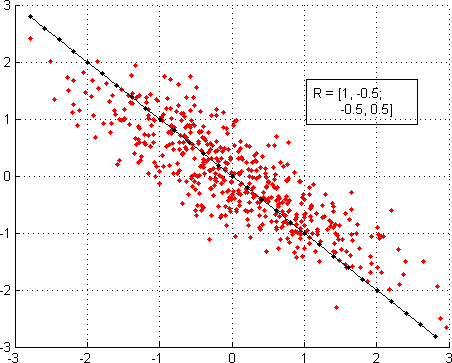
\includegraphics[width=1\linewidth]{pic/normal_our_5}
    \caption{Диаграмма рассеяния случайных величин, распределенных по нормальному закону,
      при $ R = \big[1, -0.5, -0.5, 0.5 \big] $
  }
  \label{pic:normal_end}
  \end{minipage}
\end{figure}

\newpage 

\subsection{Моделирование двумерных случайных величин, \\ 
  c распределением, равным произведению одномерных \\
  хи-квадрат раcпределений}

Диаграммы рассеяния случайных величин c распределением, 
равным произведению одномерных хи-квадрат раcпределений~\ref{pic:hi_start}--\ref{pic:hi_end}.

\begin{figure}[h!]
  \begin{minipage}[h!]{0.47\linewidth}
    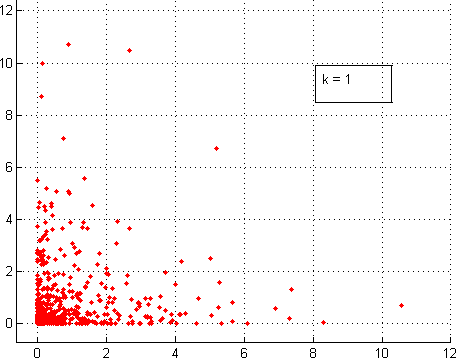
\includegraphics[width=1\linewidth]{pic/hi_our_1}
    \caption{Случайные величины, полученные по реализованному алгоритму,
      при $ k = 1 $
  }
    \label{pic:hi_start}
  \end{minipage}
  \hfill
  \begin{minipage}[h!]{0.47\linewidth}
    \vspace{4mm}
    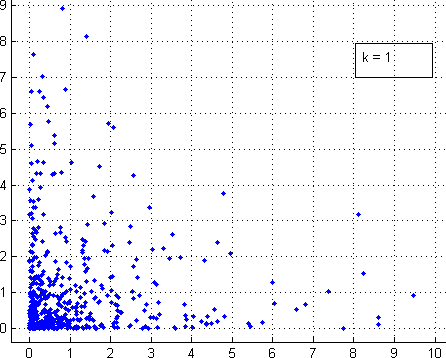
\includegraphics[width=1\linewidth]{pic/hi_matlab_1}
    \caption{Случайные величины, полученные средствами Matlab,
      при $ k = 1 $
    }
  \end{minipage}
\end{figure}

\begin{figure}[h!]
  \begin{minipage}[h!]{0.47\linewidth}
    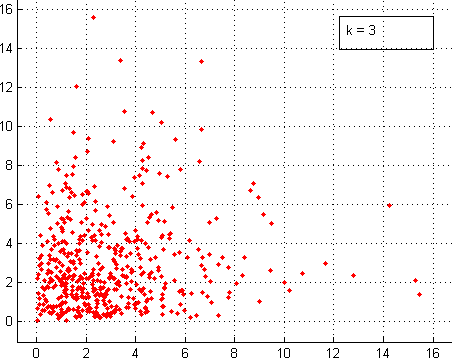
\includegraphics[width=1\linewidth]{pic/hi_our_3}
    \caption{Случайные величины, полученные по реализованному алгоритму,
      при $ k = 3 $
  }
  \end{minipage}
  \hfill
  \begin{minipage}[h!]{0.47\linewidth}
    \vspace{4mm}
    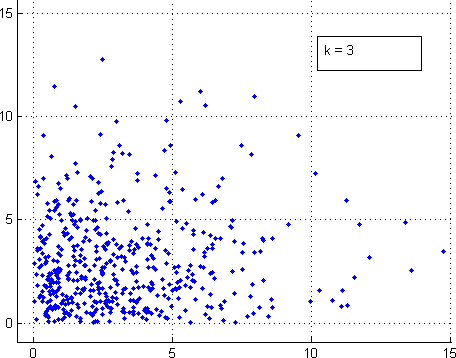
\includegraphics[width=1\linewidth]{pic/hi_matlab_3}
    \caption{Случайные величины, полученные средствами Matlab,
      при $ k = 3 $
    }
  \end{minipage}
\end{figure}

\begin{figure}[h!]
  \begin{minipage}[h!]{0.47\linewidth}
    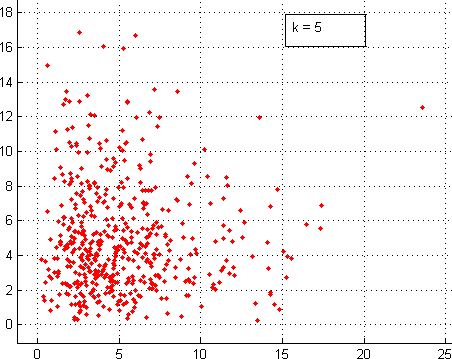
\includegraphics[width=1\linewidth]{pic/hi_our_5}
    \caption{Случайные величины, полученные по реализованному алгоритму,
      при $ k = 5 $
  }
  \end{minipage}
  \hfill
  \begin{minipage}[h!]{0.47\linewidth}
    \vspace{4mm}
    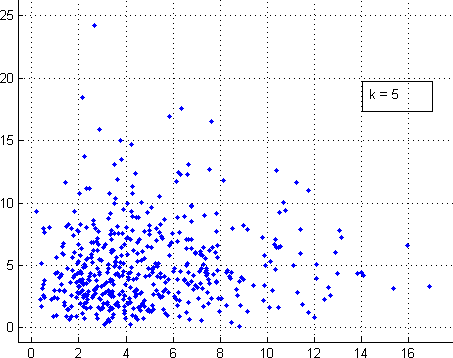
\includegraphics[width=1\linewidth]{pic/hi_matlab_5}
    \caption{Случайные величины, полученные средствами Matlab,
      при $ k = 5 $
    }
    \label{pic:hi_end}
  \end{minipage}
\end{figure}

\newpage
